\documentclass[a4paper,11pt]{scrartcl}
\usepackage[utf8]{inputenc}
\usepackage[english]{babel}
\usepackage{amsmath}
\usepackage{amssymb}
\usepackage{mathtools}
\usepackage{graphicx}



\DeclarePairedDelimiter\abs{\lvert}{\rvert}
\DeclarePairedDelimiter\norm{\lVert}{\rVert}


\title{Numerical Simulation of Fluids - Assignment 06}

\author{Jan H\"onig}


\date{\today}

\begin{document}

\maketitle


\section{Task 1 (Theory)}
\subsection{}
Momentum equation:  $\Delta u = \nabla p$

$ \Rightarrow
   \begin{pmatrix}
      \frac{\partial^2 u}{\partial x^2} + \frac{\partial^2 u}{\partial y^2} \\
      \frac{\partial^2 v}{\partial x^2} + \frac{\partial^2 v}{\partial y^2} \\
   \end{pmatrix}
   =
   \begin{pmatrix}
      \frac{\partial p}{\partial x} \\
      \frac{\partial p}{\partial y} \\
   \end{pmatrix}
$
\begin{enumerate}
   \item $\frac{\partial^2 u}{\partial x^2} + \frac{\partial^2 u}{\partial y^2} = \frac{\partial p}{\partial x}$
   \item $\frac{\partial^2 v}{\partial x^2} + \frac{\partial^2 v}{\partial y^2} = \frac{\partial p}{\partial y}$
\end{enumerate}

Continuity equation: $\nabla \cdot u = 0$

$\frac{\partial u}{\partial x} + \frac{\partial v}{\partial y} = 0$

\subsection{Discretization}
Momentum equations:
\begin{enumerate}
   \item $\frac{u_{i+1,j} - 2u_{i,j} + u{i-1,j}}{(\partial x^2)} + \frac{u_{i,j+1} - 2u_{i,j} + u_{i,j-1}}{(\partial y^2)} = \frac{p_{i+1,j} - p_{i,j}}{\partial x}$
   \item $\frac{v_{i+1,j} - 2v_{i,j} + v{i-1,j}}{(\partial x^2)} + \frac{v_{i,j+1} - 2v_{i,j} + v_{i,j-1}}{(\partial y^2)} = \frac{p_{i+1,j} - p_{i,j}}{\partial y}$
\end{enumerate}

Continuity equation:

$ \frac{u_{i+1,j} - u_{i,j}}{\partial x} + \frac{v_{i,j+1} - v_{i,j}}{\partial y} = 0 $

\section{Task 2 (Programming)}

\subsection{a) (with b) and c))}

Matrix is in file "matrix.txt"
\subsection{e)}

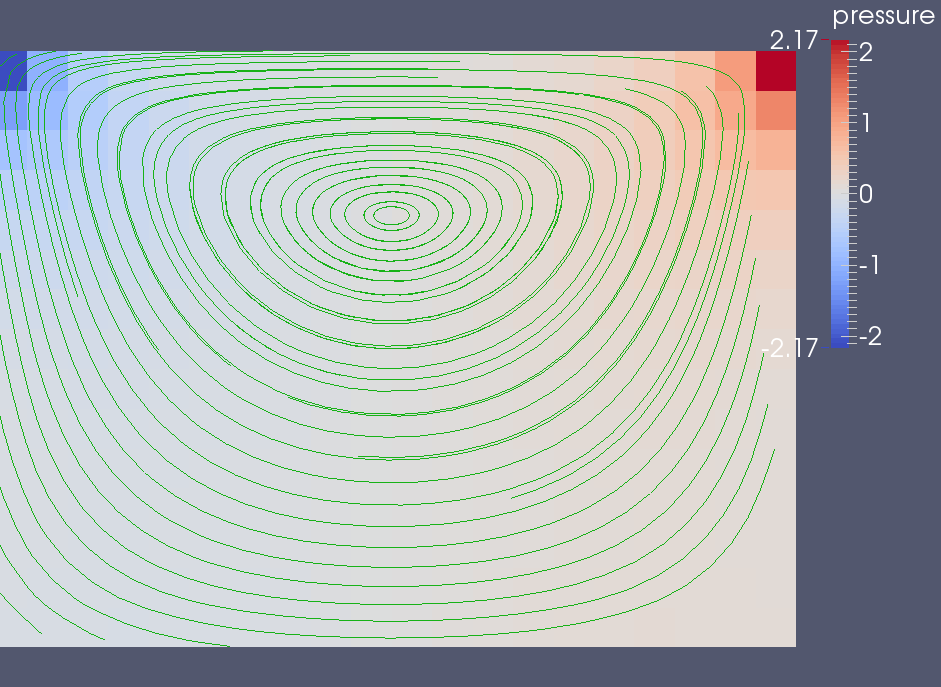
\includegraphics[width=\textwidth]{stokes.png}


\section{Task 3 (Theory)}

\[
   \begin{pmatrix}
      A & B \\
      B^T & 0 \\
   \end{pmatrix} \cdot \begin{pmatrix}
      u\\
      v\\
   \end{pmatrix}  = \begin{pmatrix}
      g\\
      0\\
   \end{pmatrix}
   \]
\[
   \begin{pmatrix}
      I & 0\\
      B^T A^{-1} & I \\
   \end{pmatrix}
   \begin{pmatrix}
      A & B \\
      B^T & 0 \\
   \end{pmatrix} \cdot \begin{pmatrix}
      u\\
      v\\
   \end{pmatrix}  = 
   \begin{pmatrix}
      I & 0\\
      B^T A^{-1} & I \\
   \end{pmatrix}
   \begin{pmatrix}
      g\\
      0\\
   \end{pmatrix}
   \]
\[
   \begin{pmatrix}
      A & B \\
      0 & B^TA{-1}B \\
   \end{pmatrix} \cdot \begin{pmatrix}
      u\\
      v\\
   \end{pmatrix}  = \begin{pmatrix}
      g\\
      B^TA^{-1}g\\
   \end{pmatrix}
   \]



\end{document}
